\thispagestyle{cackithitoannone}
\pagestyle{cackithitoan}
\everymath{\color{cackithi}}
\graphicspath{{../cackithi/pic/}}
\begingroup
\AddToShipoutPicture*{\put(0,616){
\includegraphics[width=19.3cm]{../bannercackithi}}}
\AddToShipoutPicture*{\put(150,575){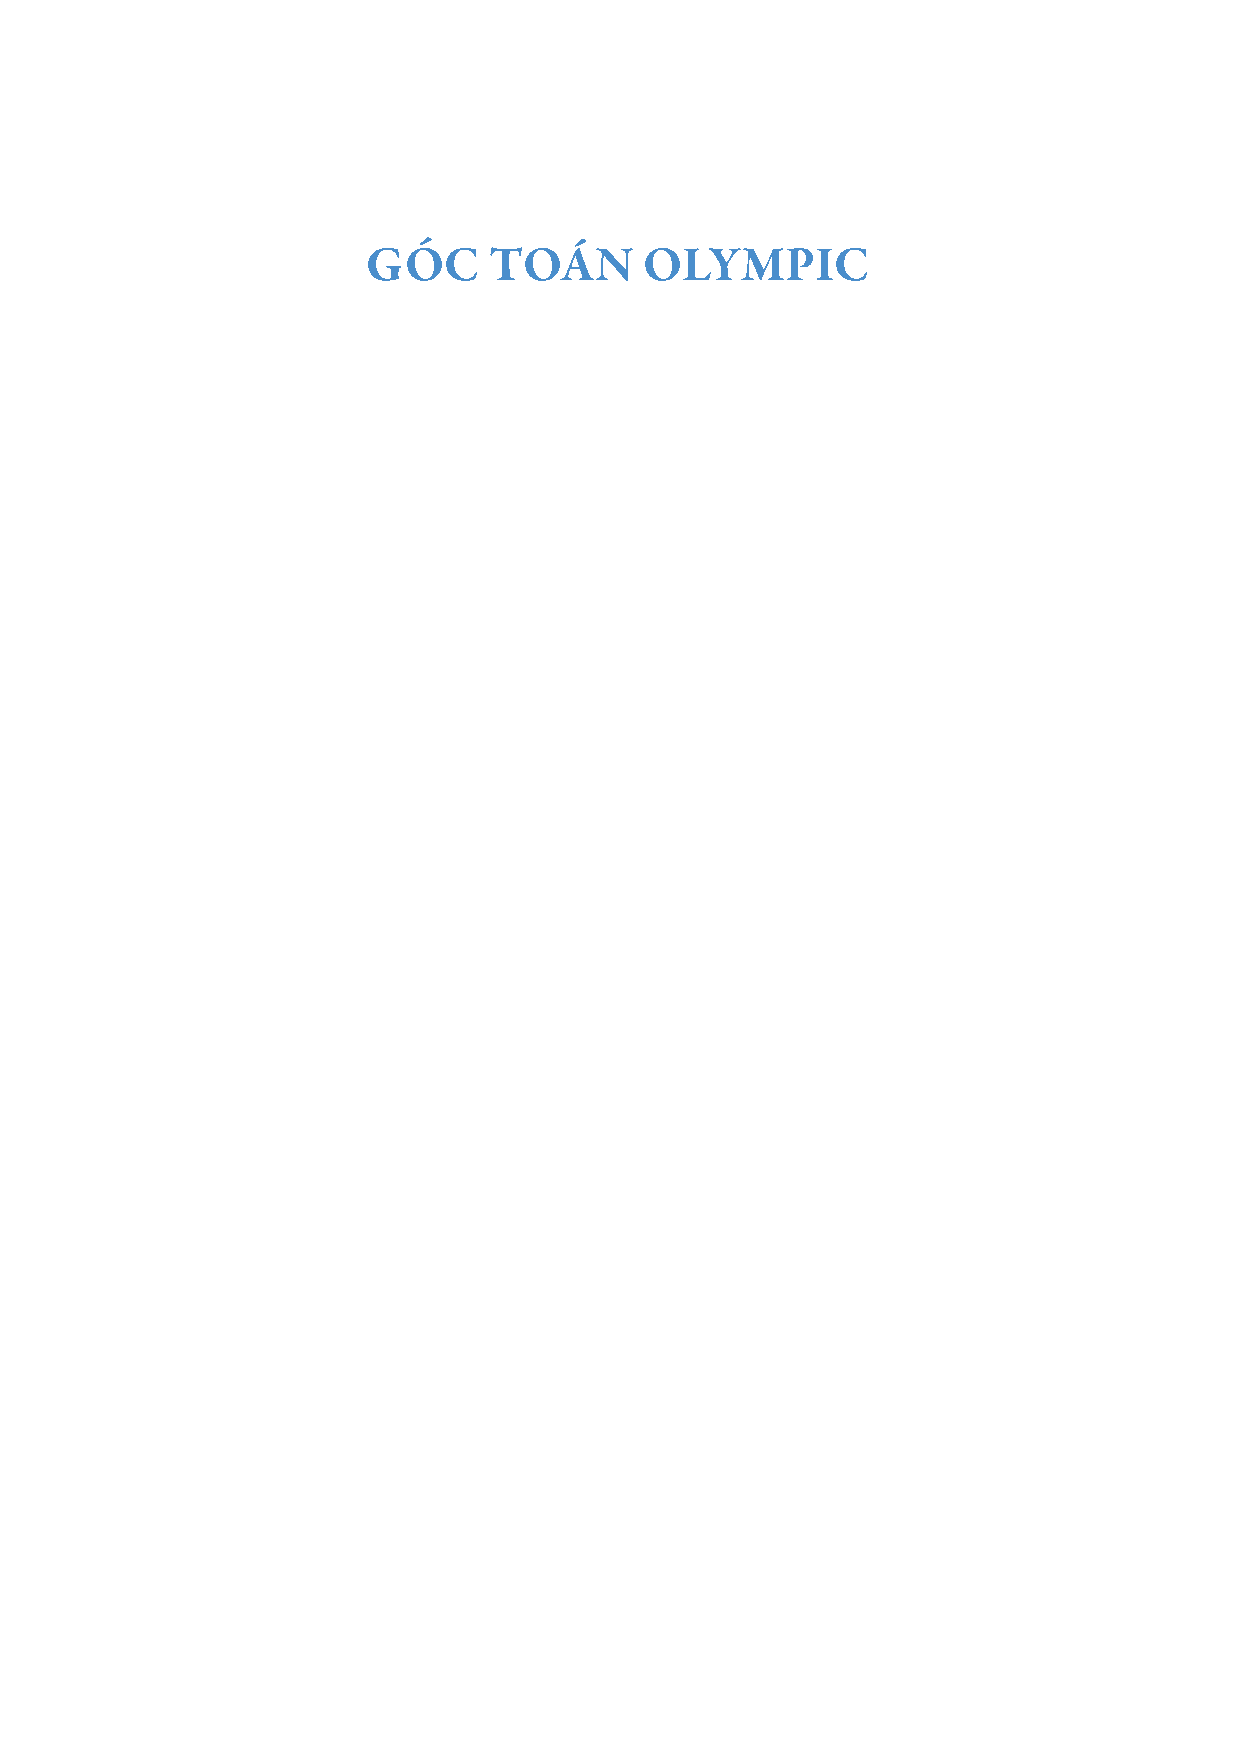
\includegraphics[scale=1]{../tieude1.pdf}}}
\centering
\endgroup
\vspace*{125pt}

\begin{multicols}{2}
	Trong phần đầu chuyên mục, chúng tôi sẽ trình bày lời giải của các bài toán trong kỳ thi Olympic Toán học trẻ khối Pháp ngữ năm $2022$ đăng trong số báo $3/2022$. 
	\begin{figure}[H]
		\vspace*{-5pt}
		\centering
		\captionsetup{labelformat= empty, justification=centering}
		
\includegraphics[width= 1\linewidth]{gocolympic}
%		\caption{\small\textit{\color{}.}}
		\vspace*{-15pt}
	\end{figure}
	{\bf\color{cackithi} OC$\pmb{34.}$} Tìm tất cả các số nguyên dương $n$ sao cho $ \lfloor \sqrt{n}\rfloor $ là ước của $n.$ 
	\vskip 0.1cm
	\textit{Chú ý}: $ \lfloor x \rfloor $ ký hiệu phần nguyên của một số thực $x,$ được định nghĩa là số nguyên lớn nhất nhỏ hơn hoặc bằng $x.$ Ví dụ: $ \lfloor 1.4 \rfloor =1$, $ \lfloor 2 \rfloor=2,$ và  $ \lfloor 2.9 \rfloor= 2.$  
	\vskip 0.1cm 
	\textit{Lời giải.} Đặt $k:=\lfloor \sqrt{n}\rfloor,$ theo định nghĩa phần nguyên ta có $k\le \sqrt{n}< k+1.$ Do đó $k^2\le n < (k+1)^2$, ta nhận được $k^2\le n\le k^2+2k$. Như vậy $k\le \frac{n}{k}\le k+2.$ Do $k$ là ước của $n$, ta suy ra $\frac{n}{k}$  bằng  một trong ba giá trị $k, k+1$ hoặc $k+2$. Tức là $n$ có phải có dạng $k^2, k(k+1)$ hoặc $k(k+2)$. Dễ đang kiểm tra các số $n$ có dạng này đều thỏa mãn điều kiện đầu bài.  
	\vskip 0.1cm
	\textit{Chú ý}: từ bất đẳng thức $k^2\le n\le k^2+2k$ ta cũng có thể lý luận như sau.  Do $0\le n-k^2\le 2k$ và $n-k^2$ là bội của $k$ nên $n-k^2$ nhận một trong ba giá trị $0, k$ hoặc $2k.$ Từ đó cũng nhận được kết luận như trên.  
	\vskip 0.1cm
	{\bf\color{cackithi} OC$\pmb{35.}$} Cho một bảng ô vuông cỡ $n \times n$ với $n\ge 1$. Aya muốn tô màu  $k$ ô của bảng  sao cho chỉ có duy nhất một cách để đặt  $n$ đồng xu trên các ô vuông được tô màu sao cho không có hai đồng xu nào nằm trên cùng một hàng hoặc cột. Hỏi giá trị tối đa có thể của $k$  là bao nhiêu?
	\vskip 0.1cm
	\textit{Lời giải.} Giả sử Aya tô màu tất cả $\frac{n(n+1)}{2}$ ô nằm từ đường chéo trở lên như trong hình vẽ minh họa. Ta đánh số các hàng và cột như trong hình vẽ.  Từ giả thiết, ta suy ra trên mỗi hàng và mỗi cột phải có đúng một đồng xu của Aya. Như vậy, trên hàng cuối phải đặt đồng xu vào cột $1$. Do đó trên hàng $n-1$ chỉ có một lựa chọn duy nhất là đặt đồng xu vào cột $2$. Tiếp  tục lý luận như vậy ta suy ra chỉ có một cách duy nhất là đặt các đồng xu lên đường chéo như trong hình vẽ.
	\begin{figure}[H]
		\vspace*{-5pt}
		\centering
		\captionsetup{labelformat= empty, justification=centering}
		\begin{tikzpicture}[scale=0.85]
			\filldraw[cackithi!50] (0,0) rectangle (1,5);
			\filldraw[cackithi!50] (1,1) rectangle (2,5);
			\filldraw[cackithi!50] (2,2) rectangle (3,5);
			\filldraw[cackithi!50] (3,3) rectangle (4,5);
			\filldraw[cackithi!50] (4,4) rectangle (5,5);
			\draw (0,0) grid (5,5);	
			\draw [fill=white] (0.5,0.5) circle (6pt);	
			\draw [fill=white] (1.5,1.5) circle (6pt);	
			\draw [fill=white] (2.5,2.5) circle (6pt);	
			\draw [fill=white] (3.5,3.5) circle (6pt);	
			\draw [fill=white] (4.5,4.5) circle (6pt);		
			\draw (-0.5,0.5) node{$n$};
			\draw (-0.5,3.5) node{$2$};
			\draw (-0.5,4.5) node{$1$};
			\draw (0.5,5.5) node{$1$};
			\draw (1.5,5.5) node{$2$};
			\draw (4.5,5.5) node{$n$};
		\end{tikzpicture}
		\vspace*{-5pt}
	\end{figure}
	Giả sử Aya có thể tô màu $k$ thỏa mãn đầu bài. Nhận xét rằng khi đổi chỗ các hàng của bảng thì tập các ô được tô màu vẫn thỏa mãn đầu bài. Ta có thể đổi chỗ các hàng để $n$ ô chứa đồng xu là các ô đường chéo như trong hình vẽ bên dưới. Với các ô nằm ngoài đường chéo ta chia thành $\frac{n(n-1)}{2}$ cặp đối xứng nhau qua đường chéo. Nếu có một cặp mà cả $2$ ô trong đó đều được tô màu thì ta có thể chuyển $2$ đồng xu sang $2$ ô này như hình vẽ mà $n$ đồng xu vẫn nằm trên $n$ hàng và $n$ cột phân biệt. Điều này mâu thuẫn với giả thiết rằng chỉ có duy nhất một cách xếp $n$ đồng xu vào các ô được tô màu. 
	\vskip 0.1cm
	Như vậy trong mỗi cặp chỉ có tối đa một ô được tô màu và ta nhận được $k\le n+ \frac{n(n-1)}{2}=\frac{n(n+1)}{2}.$ Do đó giá trị lớn nhất của $k$ thỏa mãn đầu bài là $\frac{n(n+1)}{2}.$
	\begin{figure}[H]
		\vspace*{-5pt}
		\centering
		\captionsetup{labelformat= empty, justification=centering}
		\begin{tikzpicture}[scale=0.85]
			\filldraw[cackithi!50] (0,0) rectangle (1,1);
			\filldraw[cackithi!50] (1,1) rectangle (2,2);
			\filldraw[cackithi!50] (2,2) rectangle (3,3);
			\filldraw[cackithi!50] (3,3) rectangle (4,4);
			\filldraw[cackithi!50] (4,4) rectangle (5,5);
			\filldraw[cackithi!50] (1,4) rectangle (2,5);
			\filldraw[cackithi!50] (4,1) rectangle (5,2);
			\draw[-stealth, red] (1.5,1.8) -- (1.5,4.2);
			\draw[-stealth, red] (4.5,4.2) -- (4.5,1.8);
			\draw (0,0) grid (5,5);	
			\draw [fill=white] (0.5,0.5) circle (6pt);	
			\draw [fill=white] (1.5,1.5) circle (6pt);	
			\draw [fill=white] (2.5,2.5) circle (6pt);	
			\draw [fill=white] (3.5,3.5) circle (6pt);	
			\draw [fill=white] (4.5,4.5) circle (6pt);		
			\draw (-0.5,0.5) node{$n$};
			\draw (-0.5,3.5) node{$2$};
			\draw (-0.5,4.5) node{$1$};
			\draw (0.5,5.5) node{$1$};
			\draw (1.5,5.5) node{$2$};
			\draw (4.5,5.5) node{$n$};
		\end{tikzpicture}
		\vspace*{-5pt}
	\end{figure}
	{\bf\color{cackithi} OC$\pmb{36.}$} Cho tam giác $ABC$ và $D$ là giao điểm của đường phân giác của góc $\angle BAC$ và đường trung trực của cạnh $AC$. Đường thẳng  đi qua $B$ và song song với $AC$, cắt đường thẳng $AD$ tại $X$. Đường thẳng đi qua $B$ và song song với $CX$, cắt đường thẳng $AC$ tại $Y$. Đường tròn ngoại tiếp tam giác $ABY$ cắt đường thẳng $BX$ tại $E.$ Chứng minh rằng ba điểm $C$ , $D$ và $E$ thẳng hàng.
	\vskip 0.1cm
	\textit{Lời giải.} Do bốn điểm $A, Y, B, E$ cùng nằm trên một đường tròn ta có $\angle  AYB +\angle AEB = 180^\circ$. Mặt khác do $YB$ song song với $CX$ nên ta cũng có $\angle AYB = \angle ACX$. Từ đó ta suy ra $\angle AEB + \angle ACX = 180^\circ$, tức là tứ giác $EACX$ nội tiếp đường tròn. Ta thu được
	\begin{align*}
		\angle ACE = \angle AXE. \tag{$1$}
	\end{align*}
	Mặt khác do $AC$ song song với $BX,$ ta có 
	\begin{align*}
		\angle AXE = \angle DAC. \tag{$2$}
	\end{align*}  
	Hơn nữa do $D$ thuộc trung trực của cạnh $AC$ nên
	\begin{align*}
		\angle DAC= \angle ACD. \tag{$3$}
	\end{align*}
	Từ ($1$), ($2$) và ($3$) ta thu được $\angle ACE = \angle ACD$. Do đó $C, D$ và $E$ thẳng hàng.
	\begin{figure}[H]
		\vspace*{-5pt}
		\centering
		\captionsetup{labelformat= empty, justification=centering}
		\begin{tikzpicture}[cackithi,scale=0.75]
			\draw  (-1,4)-- (0,0);
			\draw  (0,0)-- (3,0);
			\draw  (3,0)-- (-1,4);
			\draw  (3,0)-- (2.91547594742265,-2.91547594742265);
			\draw  (-2.3873012632301998,1.52817468419245) circle (2.8345238024802684cm);
			\draw  (-3.9154759474226495,3.9154759474226495)-- (2.91547594742265,-2.91547594742265);
			\draw  (0.08452405257735007,2.91547594742265)-- (0,0);
			\draw  (2.91547594742265,-2.91547594742265)-- (-1,4);
			\draw [dashed] (3,0)-- (-3.9154759474226495,3.9154759474226495);
			\draw [fill=white] (-1,4) circle (1.5pt);
			\draw (-0.8652270775932397,4.351733470633533) node {$A$};
			\draw [fill=white] (0,0) circle (1.5pt);
			\draw (-0.44768706482769755,0.026018938382523393) node {$B$};
			\draw [fill=white] (3,0) circle (1.5pt);
			\draw (3.3435762510834244,0.04272053889314506) node {$C$};
			\draw [fill=white] (0.44603207010313306,1.446032070103133) circle (1.5pt);
			\draw (0.7514249709158204,1.6460741879128244) node {$D$};
			\draw [fill=white] (2.91547594742265,-2.91547594742265) circle (1.5pt);
			\draw (3.3101730500621813,-2.7631483468912936) node {$X$};
			\draw [fill=white] (0.08452405257735007,2.91547594742265) circle (1.5pt);
			\draw (0.2203769555971698,3.249427836932504) node {$Y$};
			\draw [fill=white] (-3.9154759474226495,3.9154759474226495) circle (1.5pt);
			\draw (-4.105337576653846,4.301628669101668) node {$E$};
		\end{tikzpicture}
		\vspace*{-10pt}
	\end{figure}
	Trong phần cuối của chuyên mục kỳ này, chúng tôi sẽ giới thiệu với bạn đọc ba bài toán trong kỳ thi Olympic Toán học trẻ của Áo năm $2022$. Các bài toán này phù hợp với trình độ học sinh lớp $7-9$.
	\vskip 0.1cm
	{\bf\color{cackithi} OC$\pmb{43.}$} Người ta muốn lát kín một bảng ô vuông kích thước $2\times 13$ ($2$ hàng, $13$ cột) bằng các tấm bìa kích thước $1\times 2$ và $1\times 3$ sao cho các tấm bìa không được chồng lên nhau hay phủ ra ngoài bảng. Có bao nhiêu cách lát nếu ta được phép xoay các tấm bìa nhưng cạnh dài của tất cả các tấm đều phải song song với nhau? (số lượng mỗi tấm không hạn chế).   
	\vskip 0.1cm
	{\bf\color{cackithi} OC$\pmb{44.}$} Cho đoạn thẳng $AB$ với trung điểm $M$. Dựng nửa đường tròn tâm $M$, đường kính $AB$. Cho $P$ là một điểm trên nửa đường tròn ($P$ khác với $A, B$)  và $Q$ là trung điểm của cung  $AP$. Gọi giao điểm của đường thẳng $BP$ với đường thẳng đi qua $M$ song song $PQ$ là  $S$.
	Chứng minh rằng $PM = PS.$
	\vskip 0.1cm
	{\bf\color{cackithi} OC$\pmb{45.}$} Tìm tất các các số nguyên tố $p, q$ và $r$ thỏa mãn $p +q^2=r^4$.
\end{multicols}
